
\section{SEAM4US project}
\label{sec:seam4us}
The aim of SEAM4US "is to develop advanced technologies for optimal and scalable control of metro stations"~\cite{SEAM4US_Website}.

% For optimal control, a predictive control architecture was developed. 
% The control architecture proactively perform energy management tasks and controls the metro station subsystems, taking different passenger densities into account~\cite{ansuini_models_2013}. 
% Also situations taking place in the future are considered by utilizing, beside others, the passengers prediction model. 
% The passenger prediction model predicts the count of persons in a certain section, on a certain time in the future.

The SEAM4US consortium consists of nine partners from six different EU countries, namely Cofely Italia Spa (Italy, Energy-efficient system management), Universita Politecnica Delle Marche (Italy, Building and environmental physics construction, Universitat Politecnica De Catalunya (Spain, Building and environmental physics and construction), Fraunhofer-Gesellschaft zur Foerderung der Angewandten Forschung E.V (Germany, middleware), Teknologian Tutkimuskeskus VTT (Finland, middleware), University of Kassel (Germany, User and agent-based scheduling modeling), Almende B.V. (Netherlands, User and agent-based scheduling modeling), CNet Svenska AB (Sweden, System integrator) and Transports Metropolitans De Barcelona Sa (Spain, Metro network operator).

The control architecture, the prediction models as well as hardware components compose the SEAM4US system, which is installed in a pilot station in Barcelona (Spain). The following section gives more details about the pilot station.


\section{Pilot Station "Passeig de Gr\`{a}cia - Line 3"}
\label{sec:station}

%TODO http://www.tmb.cat/en/detall-linia-metro/-/linia/L3/327
The SEAM4US system is implemented in the pilot station Passeig de Gr\`{a}cia - Line~3~(PdG-L3), which is a station within TMBs metro network in Barcelona (Figure~\ref{fig:PdG_entranceExit}). 
This section describes the station in more detail.

In general, a metro network consists of one or more metro lines. 
Each line has a defined railway with a given number of stops to allow passengers to get on or off the trains. 
\marginpar{
\begin{figure}%[htbp]
  \begin{center}
  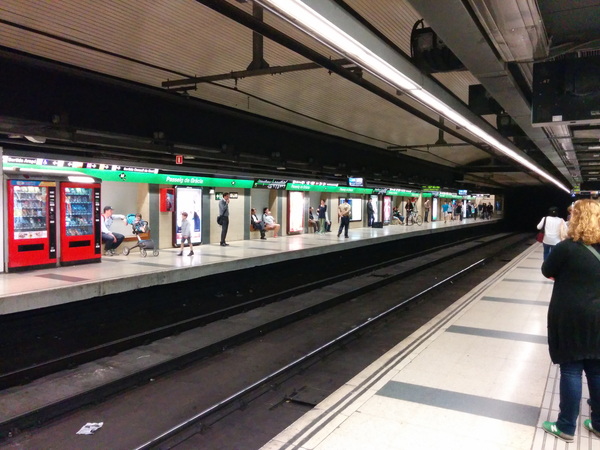
\includegraphics[width=\marginparwidth]{Figures/resized_PdG-L3_platform.jpg} 
  \caption{PdG-L3 Plattforms. \cite{TMB_2014}}
  \label{fig:PdG-L3_platforms}
  \end{center}
\end{figure}
}
Each of these stops is called "line station". 
In contrast, a "metro station" represents the architecture through which passengers get underground and into a line station. Metro station and line station can be the same physical entity, but it is possible that a metro stations holds more than one line stations.
\marginpar{
\begin{figure}%[htbp]
  \begin{center}
  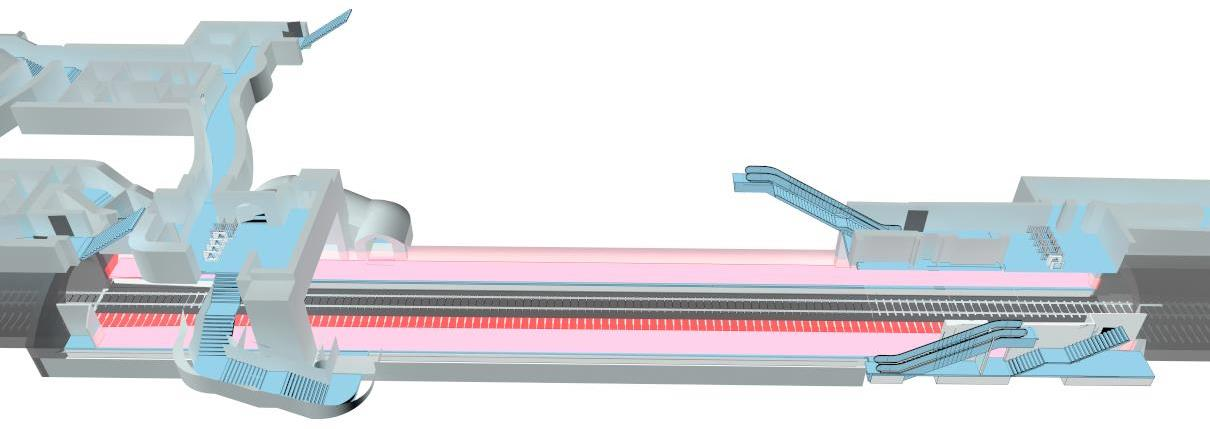
\includegraphics[width=\marginparwidth]{Figures/PdG-L3_schematic2.jpg} 
  \caption{PdG-L3 schematic representation.~\cite{TMB_2014}}
  \label{fig:PdG-L3_schematic}
  \end{center}
\end{figure}
}
\marginpar{
\begin{figure}%[htbp]
  \centering
  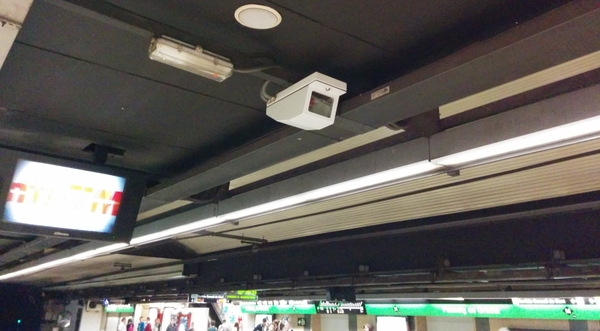
\includegraphics[width=\marginparwidth]{Figures/resized_PdG-L3_CCTVcamera_platform.jpg}
  \caption{CCTV camera in PdG-L3 platform. \cite{TMB_2014}}
  \label{fig:PdG-L3_CCTVcamera_platform}
\end{figure}
}
\marginpar{
\begin{figure}%[htbp]
  \centering
  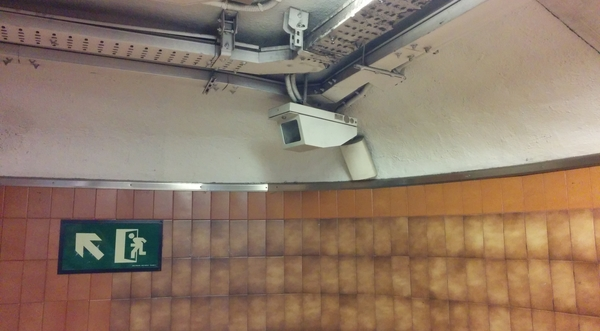
\includegraphics[width=\marginparwidth]{Figures/resized_PdG-L3_CCTVcamera_transitArea.jpg}
  \caption{CCTV camera in a PdG transit area. \cite{TMB_2014}}    
  \label{fig:PdG-L3_CCTVcamera_transitArea}
\end{figure}
}

%\marginpar{
%\begin{figure}%[htbp]
%  \begin{center}
%  \subfigure[Camera in a PdG transit area. \cite{TMB_2014}] {
%    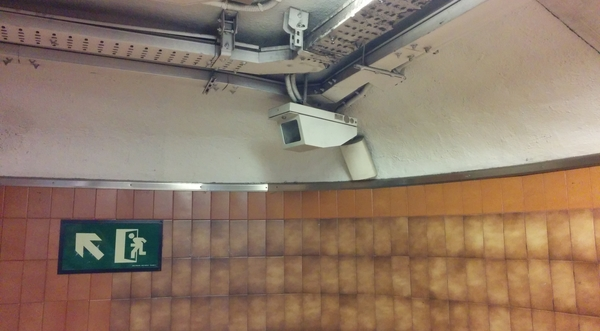
\includegraphics[width=\marginparwidth]{Figures/resized_PdG-L3_CCTVcamera_transitArea.jpg}
%    \label{fig:PdG-L3_CCTVcamera_transitArea}
%  }
%  \hfill
%  \subfigure[Camera in PdG-L3 platform. \cite{TMB_2014}] {
%    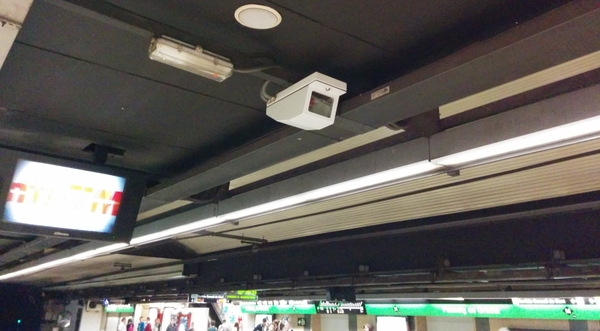
\includegraphics[width=\marginparwidth]{Figures/resized_PdG-L3_CCTVcamera_platform.jpg}
%    \label{fig:PdG-L3_CCTVcamera_platform}
%  }
%  \caption{Installed cameras}
%  \label{fig:PdG-L3_CCTVcameras}
%  \end{center}
%\end{figure}
%}

The metro station Passeig de Gr\`{a}cia~(PdG) was chosen as a representative station for the SEAM4US project.
It is located in the iconic and touristic part of Barcelona. Some popular buildings designed by Antoni Gaud\'{i} (Casa Batll\`{o}, Casa Mil\`{a}) as well as the city's most renown and exclusive boutiques are in the proximity.
The metro station is one of the oldest of the Barcelona metro network. 
First opened in December 1924, as station for Line~3~(L3), nowadays PdG holds three different line stations: Line~2, Line~3, and Line~4. The line stations were built in three different periods, using different construction technologies. 
All line stations have been refurbished a few times since 1924, and new equipment has been added recently.
Depending on the weekday PdG is open 19~hours, 21~hours, or 24~hours. 
Between Monday and Thursday PdG service starts at 5:00 and ends at 24:00 (19~hours). Friday service starts at 5:00 and ends at 2:00 (21~hours). On Saturday service starts at 5:00 too but remain the entire night and day until Sunday midnight.

PdG-L3 was as pilot station selected since it turned out to be representative for many stations within TMBs metro network~\cite{TMB_2014}. 
The count of fans, escalators, and the platform schema is comparable to other stations. 
Moreover, PdG-L3 is a crowded station which have low-rate usage hours as well. 
Therefore, a wide range of data is available, that allows to test with very busy peak hours as well as with off-peaks.

% \subsection{Spaces}
%\label{subsec:PdG-L3_spaces}

The line station PdG-L3 consists of private (staff only) and public spaces. 
Private spaces such as technical rooms or staff dependencies are not part of the investigation of the SEAM4US project, whereas public spaces, such as halls, transit areas, accesses to the platforms, and platforms are, in the focus for the energy efficient control.
The platforms are an essential part of (every) line station, since it allows passengers to leave and enter the trains. 
For the passenger model it is essential because every passenger who uses the line station is visible here. 
Figure~\ref{fig:PdG-L3_platforms} depicts the platform. 


%To leave the platforms, several escalators are available. Figure~\ref{fig:PdG-L3_escalator} depicts exemplarily an escalator.
%\begin{figure}%[htbp]
%  \centering
%  \includegraphics[width=\linewidth]{Figures/PdG-L3_escalator.jpg} 
%  \caption{Escalator in PdG-L3 for leaving the platform. \cite{TMB_2014}}
%  \label{fig:PdG-L3_escalator}
%\end{figure}

A schematic representation of PdG-L3 is drawn in Figure~\ref{fig:PdG-L3_schematic}, where the platforms are highlighted in red. At the beginning and end of the platforms, the accesses to the platforms are visible.



% \subsection{CCTV System}
%\label{subsec:CCTVSystem}

Throughout the station a Closed Circuit Television~(CCTV) surveillance system is installed. 
20~CCTV~cameras on different locations provide images for security reasons. 
Figure~\ref{fig:PdG-L3_CCTVcamera_platform} and Figure~\ref{fig:PdG-L3_CCTVcamera_transitArea} show exemplary CCTV cameras on the platform as well as in the transit area.

The CCTV~system provides the basis for the predictive passenger model. In the following, the data extraction is explained.


\section{Count of persons extraction}
\label{sec:PassengerDensityDataExtraction}

The SEAM4US system utilizes a prediction model for proactively controlling the subsystems.
Besides others, the passenger model is a part of the predictive controlling architecture.
To predict count of persons for a point in the future, the model utilizes the output of the CCTV monitoring system. 
The count of persons is extracted by enhancing the CCTV~system with image processing.

Whenever camera pictures are processed privacy issues are tackled. In order to ensure the passengers privacy several design constraints were defined:

\begin{enumerate}\setlength{\itemsep}{-2pt}
  \item All CCTV images are processed within the station.
  \item All CCTV images are processed "on the fly". For the purpose of count of persons extraction, no CCTV image is saved.
  \item The image processing is performed on a separate computer, which is not connected to other TMB Systems and is only accessible via a dedicated VPN connection.
  \item The image processing works without human interaction.
  \item The image data is filtered to avoid recognisability of individuals.
  \item The image processing results are transmitting only in terms of integer numbers to the database.
\end{enumerate}

With respect to these design constraints, the count of persons extraction was implemented. The workflow is described briefly in the following.
\marginpar{
\begin{figure}%[htbp]
  \begin{center}
  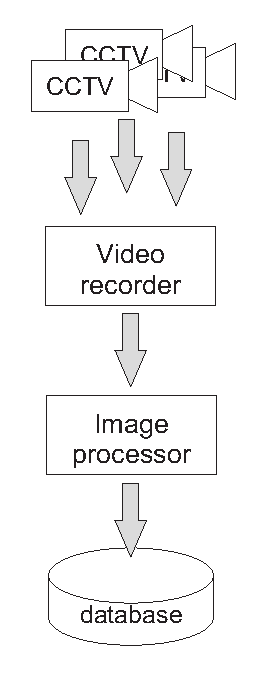
\includegraphics[width=\marginparwidth]{Figures/imageProcessing2.pdf} 
  \caption{Gathering count of persons out of the camera images.}
  \label{fig:CCTVimageProcessing}
  \end{center}
\end{figure}
}

First, the video streams extracted from all cameras are combined into one single video stream by a video recorder. 
The video recorder creates a carousel video composed of intervals for the individual camera, appearing in a predefined order. 
The duration of the camera intervals is set to 3~seconds. With 20~cameras and 3~seconds hold on each, one turn of the carousel is completed in one minute.

The video recorder is connected to a local computer and transfers the images subsequently. 
On the local computer, an extraction algorithm processes the transferred images and extracts the count of persons.
The extraction algorithm uses a combination of edge detection and background subtraction. 
% In the  following, the algorithm is described briefly.
First the algorithm separates background and foreground. 
Followed by creating the foreground mask.
Through filtering the edges of the foreground only, is extracted. 
The foreground edges are combined with the foreground mask. 
Finally, the result is refined by dilating (and then eroding) the segmented blobs.
%In parallel to the process described above, we detect the edge of the whole image by applying the Canny edge detection on the three RGB channels of the original image; the results acquired the different channels are then combined via a simple logic OR. Eventually, the intersection of this image with the dilated foreground mask  (obtained using a logic AND) allows us to extract the edges of the foreground only (see Figure 13). 
%"The last step of the crowd density detection algorithm consists in combining this last image with the foreground mask via a logic OR and to refine the result by dilating (and then eroding) the segmented the blobs."  
%All parts have been developed using the C++ OpenCV libraries.
For various reasons, for instance, occluded or damaged camera, the extraction algorithm can fail. 
In these cases, the algorithm returns the error value "-1".

The extracted count of passenger as well as date, time and the camera-ID of the image are transmitted to the database. 
The general approach is sketched in Figure~\ref{fig:CCTVimageProcessing}.


The CCTV system as well as the image processing are running 24~hours, 7~days a week. 
Each day 28800~datasets are transmitted to the database. 
Overall the database currently contains 90~days of data. 
